\chapter{Variabili Aleatorie}

\begin{figure}[H]
	\centering
	\caption{Tipi di variabili casuali}
	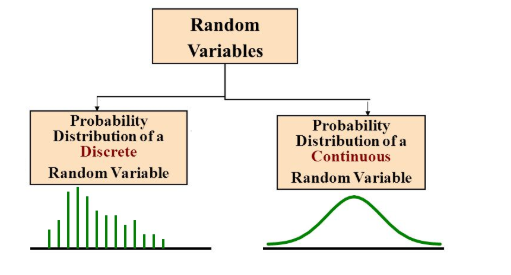
\includegraphics[]{varrandom}
\end{figure}

\section{Variabili Aleatorie Discrete}

Una variabile aleatoria (casuale o stocastica) discreta è una variabile che può assumere diversi valori in dipendenza da qualche fenomeno casuale.
Il risultato del lancio di un dado, ad esempio, è una variabile aleatoria discreta.

Prendiamo uno \textbf{spazio probabilizzabile} $ (\Omega, F) $ e una variabile aleatoria discreta $ x : \Omega \to \R $, che è una funzione continua non surgettiva. I valori di $ x $ devono essere un sottoinsieme finito di $ \R $ ovvero $ \{a_1, \dots, a_k\} $.
Vogliamo anche che $ \forall j \in [1, k] $ sia vero $ x^{-1}(a_j) = \{ \omega \in \Omega, x(\omega) = a_j\} \in F $. Utilizziamo la funzione inversa per ottenere gli elementi di $ \Omega $ su cui possiamo definire la probabilità.

Con la probabilità di tutti gli eventi definisco la densità di probabilità. Nello spazio probabilizzato $ (\Omega, F, \mathcal{P}) $ la probabilità che la variabile aleatoria assuma il valore $ a_j $ sarà $ p_j = \p{x = a_j} = \p{x^{-1}(a_j)} $, che viene detta densità di probabilità. Varranno quindi le seguenti proprietà

\begin{enumerate}
	\item $ \forall j \ldotp x^{-1} (a_j) $ sono tutti insiemi disgiunti.
	\item Essi coprono tutto $ \Omega $
\end{enumerate}

Vale che $ \sum_{j=1}^{k} p_j = 1 $. Poiché:
\[ 1 = \p{\Omega} = \p{\bigcup_{j} x^{-1}(a_j)} = \sum_{j} \p{x^{-1}(a_j)}\] 

Sia $ x : \Omega \to \{ a_1, \dots, a_k \} $ una variabile aleatoria, e sia la densità di probabilità $ p_j \geq 0 $ e anche  $ \sum_{j=1}^{k} p_j = 1 $, allora $ \p{x = a_j} = p_j $.

Preso uno spazio probabilizzabile $ (\Omega, F) $ e una variabile aleatoria $ x : \Omega \to \{ a_1, \dots, a_k \} $, supponendo che i numeri $ a_j $ siano ordinati, sia $ p_j $ la densità di probabilità, come posso ricostruire, ad esempio $ \p{x \leq a_3} $?

\[ \p{x \leq a_3} = \p{(x=a_1) \cup (x=a_2) \cup (x=a_3)} = \p{x = a_1} + \p{x = a_2} + \p{x = a_3}  \]

\paragraph{Esempio}

Voglio contare quanti 6 escono in 10 lanci di dadi.

Sia $ \Omega = \{ (1, 2, 3, 4, 5, 6)\}^{10} $, ovvero tutte le possibili parole di 10 elementi composte dai numeri da 1 a 6. Ad ogni lancio, ho $ \frac{1}{6} $ di probabilità di ottenere 6 e $ \frac{5}{6} $ di ottenere gli altri numeri. Definiamo la variabile aleatoria $ x : \Omega \to \{ 0, 1, 2, \dots, 9, 10 \} $ come il conteggio dei risultati dei lanci dove ottengo 6. Qual'è la probabilità di ottenere 3 lanci dove ho fatto 6?

\[ \p{x = 3} = \binom{10}{3} \left(\dfrac{1}{6}\right)^3 \left(\dfrac{5}{6}\right)^7 \]

% TODO spiega

\subsection{Legge di Bernoulli}
Faccio un esperimento, il risultato positivo ha probabilità $ p $, mentre il risultato negativo ha probabilità $ 1 - p $

Sia lo spazio $ \Omega = \begin{cases}
\text{successo} \to 1 \\
\text{insuccesso} \to 0
\end{cases} $

Una variabile aleatoria Bernoulliana è definita come $ x : \Omega \to \begin{cases}
p_1 = p \\ p_0 = 1 - p
\end{cases} $

\paragraph{Legge Binomiale} 
Sia $ k $ il conteggio dei successi di $ n $ esperimenti, abbiamo quindi che $ B(n,p) = x_i\{(0,1)\}^n \to \{0, \dots, n\} $. Abbiamo che la densità di probabilità Binomiale $ p_k = \p{x=k} = \binom{n}{k} p^k(1-p)^{n-k} $.

$ p_k $ è una densità? Sappiamo che $ p_k \geq 0 $ e sappiamo che $ 1 = \sum_{k} p_k $, con il binomio di Newton possiamo dimostrare che $ (a+b)^n = \sum_{k=0}^{n} \binom{n}{k} a^k b^{n-k} $. Proseguendo, abbiamo che 

\[ \sum_{k} p_k = \sum_{k=0}^{n} \binom{n}{k} p^k (1-p)^{n-k} = (p+(1-p)^n) = 1^n = 1 \]

\subsection{Somma di Variabili Aleatorie}
Lancio due dadi, uno rosso e uno nero, avremo quindi $ \Omega = \{R, N\} = \{(1,6)\}^2 $. Definisco due variabili aleatorie, $ x $ per il dado rosso dove $ x : (R, N) \to R $ e la variabile $ y : (R, N) \to N $. La densità per $ x $ sarà $ p_j = \frac{1}{6} \forall j $ mentre la densità per $ y $ sarà $ q_j = \frac{1}{6} \forall j $
Avremo che $ z = x + y $ conta la somma dei dadi. Come esercizi per casa:
\begin{enumerate}
	\item Calcolare la densità di Z
	\item Calcolare $ \p{4 \leq z \leq 6} $
\end{enumerate}

% TODO Svolgi

\subsection{Indipendenza di Variabili Aleatorie}

Due variabili aleatorie $ x_1, x_2 $ sono indipendenti se $ \forall I_1, I_2, \subseteq \R $ intervalli o semirette si ha che 

\[ \left( \p{x_1 \in I_1} \cap \p{x_2 \in I_2} \right) = \p{x_1 \in I_1} - \p{x_2 \in I_2} \]

Nell'esempio di prima $ x, z $ e $ y,z $ sono dipendenti perché dati $ I_1 = [1,2], I_2 = [3,4] $ allora si ha che $ \p{x\in I_1} = \p{x=1,2} = \frac{1}{3} $ e si ha anche $ \p{z \in I_2} = \p{2 = 3,4} = \frac{5}{36} $. Ne otteniamo che:

\[ \p{(x \in I_1) \cap (z = 3,4)} = \p{(x = 1,2, z = 3,4)} = \dfrac{4}{12} \]
